\documentclass[preprint,3p,twocolumn]{elsarticle}
%\documentclass[preprint,1p]{elsarticle}
\usepackage{graphicx}
\usepackage{mathrsfs}
\usepackage{algorithm,algorithmicx, algpseudocode}
\usepackage{amsmath,amssymb}
\usepackage{caption}
\captionsetup[table]{font=small,skip=0pt,singlelinecheck=off}

\usepackage{multicol}
\usepackage[export]{adjustbox}
\usepackage{lineno,hyperref}
\usepackage{fancyvrb}
\usepackage{bchart}
\usepackage{booktabs}
\usepackage{tikz}
\usetikzlibrary{arrows.meta,positioning,shapes.geometric,calc}
\usepackage{pgfplots}
\pgfplotsset{compat=1.18}

\modulolinenumbers[5]

\def\CircleArrow{\hbox{$\circ$}\kern-1.5pt\hbox{$\rightarrow$}}

\def\bsq#1{%both single quotes
\lq{#1}\rq}

\algnewcommand\algorithmicnot{\textbf{not}}
\algdef{SE}[IF]{IfNot}{EndIf}[1]{\algorithmicif\ \algorithmicnot\ #1\ \algorithmicthen}{\algorithmicend\ \algorithmicif}%

\journal{arXiv}

%% `Elsevier LaTeX' style
\bibliographystyle{elsarticle-num}

\let\today\relax
\makeatletter
\def\ps@pprintTitle{%
    \let\@oddhead\@empty
    \let\@evenhead\@empty
    \def\@oddfoot{\footnotesize\itshape
         {~} \hfill\today}%
    \let\@evenfoot\@oddfoot
    }
\makeatother

\newcommand{\MR}{MarketRank}
\newcommand{\FS}{Fluxscape}

\begin{document}

\begin{frontmatter}

\title{MarketRank: ranking stocks by the stationary probabilities of a Markov chain over estimated money flows, with a topological landscape view}

\author{B. Kaan Karamete\corref{cc}}

\cortext[cc]{\it Corresponding author: B. Kaan Karamete, karametebkaan@gmail.com}
\address{Graph AI LLC}

\begin{abstract}
We present \MR, a Markov-chain transition-probability solver for the stock market. Its states are stocks, its transition probabilities are the out-shares of estimated stock-to-stock dollar flows, and a stock's MarketRank score is the chain's stationary probability $\pi_i$, computed by damped power iteration. The stationary condition of the damped chain is the \emph{MarketRank Condition} $r_i=(1-p)\sum_{j}r_j\,T_{j\to i}/\sum_k T_{j\to k}+p/N$, with damping $p=0.15$; PageRank is the best-known instance of the same construction, applied to hyperlinks. Paired transactions between stocks are not public, so the flow matrix $T$ is \emph{estimated} from public daily bars. Each bar's signed dollar pressure splits net sellers' outflow over net buyers by a correlation-tilted gravity model, and the result is accumulated over the data window and pruned to a sparse graph. The engine is written in C++20 with OpenMP and gives bit-identical results for any thread count. It ranks a liquidity-ranked universe of 10,000 US tickers (about 6,200 active) from a DuckDB-catalogued Parquet lake. A 3D view, \FS, turns each frame into a landscape. Flux communities from a deterministic, warm-started Louvain become territories, which are ordered by spectral bisection along a generalized Hilbert curve and filled centre-out on a spiral. The surface is interpolated by inverse-distance weighting, smoothed by a centroidal-Voronoi-style relaxation and Gouraud-shaded. On real data the top of the ranking is the large-cap semiconductor and technology complex (MU, SNDK, NVDA, TSLA, \dots), and the landscape is stable between frames (median cell jump 0). The flows show sector structure, but the evaluated scores have no material predictive information coefficient for next-day returns. We state these limits plainly and outline calibration against observed account-level pairings from SEC Form 13F.
\end{abstract}

\begin{keyword}
\it Markov chains, stationary distribution, transition probabilities, PageRank, money flow, origin--destination estimation, community detection, spectral ordering, scattered-data interpolation
\end{keyword}

\end{frontmatter}

%% ------------------------------------------------------------------
\section{Introduction}
\label{Section:intro}

Every trading day, dollars leave some stocks and enter others. A portfolio manager who trims one position and adds to another, an index rebalance, or a sector rotation each move money \emph{from} one name \emph{to} another. If those pairings were visible, the market would be a directed, weighted graph of money flows, and a natural question would be where money \emph{concentrates} in steady state, and how that concentration \emph{rotates} from day to day.

A finite-state Markov chain~\cite{norris,kemenysnell} answers exactly this kind of question. If the states are stocks and the probability of moving from $j$ to $i$ is the share of $j$'s outflow that goes to $i$, then the chain's stationary distribution $\pi$ is the long-run fraction of money at each stock. \MR\ is a solver for that stationary distribution. Let $T_{j\to i}\ge 0$ be the dollars that moved from selling stock $j$ into buying stock $i$ over a window. The transition probability from $j$ to $i$ is the out-share $T_{j\to i}/\sum_k T_{j\to k}$. With damping $p$, the stationary condition of the damped chain is the \emph{MarketRank Condition} (MRC)
\begin{equation}
\begin{aligned}
r_i&=(1-p)\sum_{j\in B(i)}P_i(r_j)+\frac{p}{N},\\
P_i(r_j)&=r_j\,\frac{T_{j\to i}}{\sum_k T_{j\to k}},
\end{aligned}
\label{eqn:mrc}
\end{equation}
where $B(i)$ is the set of stocks that send money to $i$, $N$ the number of active stocks and $p=0.15$. Its solution $r=\pi$ is the MarketRank score. PageRank~\cite{brinpage,pagerank} is the best-known instance of the same construction: a damped chain whose transition probabilities are the out-shares of hyperlinks. MarketRank is analogous, with dollars in place of links. A stock ranks high when it receives a large share of what its senders give away, and when those senders themselves rank high. The rank is a property of the whole flow network, not of a stock's own volume.

The difficulty is that trades are anonymous: a tape shows that a stock traded, not which stock the buyer sold to fund it. \MR\ therefore \emph{estimates} $T$ from public bars, and is explicit that every downstream number inherits that estimate.

\paragraph{Contributions}
\begin{itemize}
\item \textbf{The model:} a damped Markov chain over stocks whose transition probabilities are dollar out-shares. Its stationary distribution, defined by the MRC~(\ref{eqn:mrc}), is the score. Dangling stocks are handled by teleport. A worked three-stock example reproduced by the test suite (Section~\ref{Section:model}).
\item \textbf{Flow estimation from public bars:} signed dollar pressure, a correlation-tilted gravity pairing with exact row and column totals in $O(NW)$, sparse candidate sinks, cumulative accumulation and two-sided pruning (Section~\ref{Section:flows}).
\item \textbf{A scalable deterministic engine:} C++20 and OpenMP with bit-identical results across thread counts, a CSR matrix and its transpose, and a DuckDB catalogue over a Hive-partitioned Parquet lake fed from the Alpaca SIP feed, at 10,000 tickers (Section~\ref{Section:engine}).
\item \textbf{The \FS\ landscape:} a deterministic pipeline from the flow graph to a stable, shaded 3D terrain (Section~\ref{Section:landscape}).
\end{itemize}
Section~\ref{Section:results} reports results on real data, including an evaluation that finds structure but no material predictive power, and Section~\ref{Section:limits} lists the limitations and planned work.

%% ------------------------------------------------------------------
\section{Related work}
\label{Section:related}

\paragraph{Markov chains and stationary distributions} An irreducible, aperiodic finite Markov chain has a unique stationary distribution $\pi=\pi P$, and power iteration converges to it~\cite{norris,kemenysnell}. Damping, that is mixing $P$ with a uniform jump of probability $p$, makes any chain irreducible and aperiodic, and the convergence rate is then at most $1-p$ per iteration. \MR\ is a solver for this stationary distribution, on a chain whose transition probabilities are estimated dollar out-shares.

\paragraph{PageRank as an instance} PageRank~\cite{brinpage,pagerank} is the best-known application of the same transition-probability concept. A random surfer follows out-links with probability $1-p$ and teleports with probability $p$, and dangling pages are usually redistributed uniformly. \MR\ uses the same damped chain with dollar out-shares in place of link out-shares. Like PageRank, MarketRank is a Markov-chain ranking.

\paragraph{The author's Markov-chain lineage} This work continues the author's earlier use of Markov-chain transition probabilities:
\begin{itemize}
\item an adaptive Markov chain for map matching of vehicle GPS trips~\cite{kineticamapmatching};
\item the probability-rank and PageRank graph solvers of Kinetica-Graph~\cite{kineticagraph,kinetica}.
\end{itemize}
The \MR\ solver is native C++ with no database dependency.

\paragraph{Money-flow indicators} Technical money-flow indicators combine price change and volume \emph{per stock}, so a stock's flow is a scalar with no counterparty. \MR\ keeps the same raw ingredients (return, volume, VWAP) but pairs sources with sinks, so that flow becomes an edge and the ranking a network property. Signed order-flow methods such as the Lee--Ready trade classification~\cite{leeready} sign trades from quotes; we treat them as future input (Section~\ref{Section:limits}).

\paragraph{Origin--destination estimation from marginals} Recovering a flow matrix from its row and column totals is the classic origin--destination problem of transport planning. The gravity model and its entropy-maximizing derivation~\cite{wilson} give the most probable matrix consistent with the marginals, $F_{ij}\propto O_i D_j$, optionally modulated by an impedance or affinity term. Section~\ref{Section:flows} is a singly constrained gravity model of this kind, with return correlation as the affinity.

\paragraph{Communities and spectral partitioning} Louvain~\cite{louvain} greedily maximizes modularity in two alternating phases (local moves, then aggregation). Recursive spectral bisection (RSB)~\cite{rsb} splits a graph by the sign or median of the Fiedler vector~\cite{fiedler}, the second eigenvector of the graph Laplacian; we use the normalized Laplacian~\cite{chung} of the community graph and the generalized Hilbert curve~\cite{hilbert,gilbert} to turn the spectral order into contiguous regions of a lattice.

\paragraph{Scattered-data interpolation and smoothing} Shepard's inverse-distance weighting (IDW)~\cite{shepard} interpolates scattered values with weights $d^{-q}$. Centroidal Voronoi tessellations and Lloyd's algorithm~\cite{cvt,lloyd} relax generators toward the density-weighted centroids of their cells; our display smoother borrows that density weighting. Gouraud shading~\cite{gouraud} interpolates vertex colours across triangles.

\paragraph{Double-link adjacency} The double link structure (DLS)~\cite{dls} keeps both directions of mesh adjacency so that upward and downward queries are equally cheap. The \MR\ solver keeps the transition matrix and its transpose for the same reason (Section~\ref{Section:engine}).

%% ------------------------------------------------------------------
\section{Model}
\label{Section:model}

\paragraph{Paired flow matrix} For $N$ active stocks, $T\in\mathbb{R}_{\ge 0}^{N\times N}$ holds $T_{j\to i}$, the dollars that left $j$ (net selling) and entered $i$ (net buying) over the data window, with no diagonal. Section~\ref{Section:flows} describes how $T$ is estimated.

\paragraph{Out-share functor} Row-normalizing $T$ gives the transition matrix $P_{j i}=T_{j\to i}/\sum_k T_{j\to k}$, and the functor $P_i(r_j)=r_j P_{ji}$ is the part of $j$'s rank that $j$ passes to $i$. $P$ is the transition matrix of a finite Markov chain on the stocks, and Equation~(\ref{eqn:mrc}) is the stationary condition $\pi=(1-p)\,\pi P+(p/N)\mathbf{1}$ of its damped version. The solution $r=\pi$ is the vector of stationary probabilities.

\paragraph{Damping and dangling stocks} We use $p=0.15$ ($\alpha=1-p=0.85$), solved on the active sub-index. A stock with no kept outflow is a \emph{dangling} node: its row is empty, and its mass $d$ is spread uniformly, as in PageRank, so that
\begin{equation}
\pi'=\alpha\left(\pi P+\frac{d}{N}\mathbf{1}\right)+\frac{1-\alpha}{N}\mathbf{1}.
\end{equation}
Power iteration starts from the uniform vector (warm-started from the previous bar in the pipeline) and stops when $\lVert\Delta\pi\rVert_1<10^{-10}$ or after 1000 iterations. The \emph{MarketRank score} is $\pi_i N$ (1 = average), and the \emph{heartbeat} is the pulse of the score, $\Delta\log(\pi_i N)$ between consecutive bars. Using the score rather than $\pi_i$ removes the common-mode term $-\Delta\log N$ that a change in the number of active stocks adds to every $\log\pi_i$, so a stock whose score did not move reads 0.

\paragraph{Worked example} Figure~\ref{Figure:abc} shows three stocks with six flows. Row-normalizing gives
\[
P=\begin{pmatrix}0 & 5/6 & 1/6\\ 1/6 & 0 & 5/6\\ 15/23 & 8/23 & 0\end{pmatrix}
\]
(rows and columns A, B, C). Table~\ref{Table:abc} lists the ranks after seven damped iterations from the uniform start and at convergence. B ranks first although C receives the most dollars (1.1M, against 0.9M for B): the chain counts shares, not dollars. B receives 5/6 of A's outflow and 8/23 of C's, and A, which gives most of its outflow to B, is itself fed by C's largest edge (15/23 of C's outflow). The unit test \texttt{test\_market\_rank.cpp} reproduces both rows through the solver (within $5\cdot10^{-5}$ after seven iterations and $10^{-5}$ at convergence) and through the pipeline's own accumulator and transition builder under the \MR\ preset.

\begin{figure}[t]
\centering
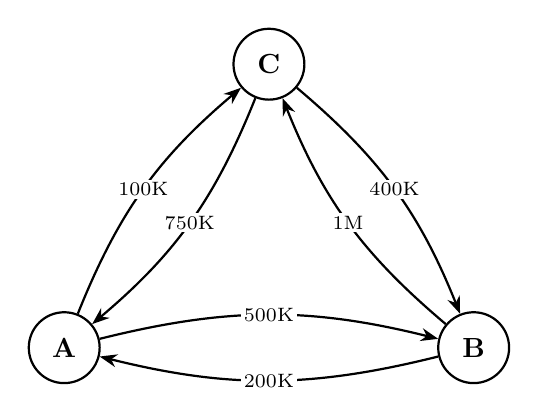
\begin{tikzpicture}[>={Stealth[length=2.2mm]},
  st/.style={circle,draw,thick,minimum size=9mm,font=\bfseries},
  fl/.style={->,thick,bend left=14},
  lb/.style={font=\scriptsize,fill=white,inner sep=1pt}]
  \node[st] (A) at (0,0) {A};
  \node[st] (B) at (5.2,0) {B};
  \node[st] (C) at (2.6,3.6) {C};
  \draw[fl] (A) to node[lb]{500K} (B);
  \draw[fl] (B) to node[lb]{200K} (A);
  \draw[fl] (A) to node[lb]{100K} (C);
  \draw[fl] (C) to node[lb]{750K} (A);
  \draw[fl] (B) to node[lb]{1M} (C);
  \draw[fl] (C) to node[lb]{400K} (B);
\end{tikzpicture}
\caption{Worked example: three stocks and six dollar flows $T_{j\to i}$ (arrow from seller $j$ to buyer $i$).}
\label{Figure:abc}
\end{figure}

\begin{table}[t]
\centering
\caption{Ranks of the worked example (Figure~\ref{Figure:abc}), $p=0.15$, uniform start.}
\label{Table:abc}
\begin{tabular}{lccc}
\toprule
 & B & C & A\\
\midrule
After 7 iterations & 0.35980 & 0.34770 & 0.29248\\
Converged & 0.36016 & 0.34665 & 0.29319\\
\bottomrule
\end{tabular}
\end{table}

%% ------------------------------------------------------------------
\section{Estimating flows from public market bars}
\label{Section:flows}

Only bars are public: for each stock and bar $t$, the close $C$, the volume $V$ and the volume-weighted average price $\mathrm{VWAP}$. The estimator below is deterministic and has no fitted parameters.

\paragraph{Pressure} With return $r_i=C_i/C_i^{-}-1$, the \MR\ preset uses dollar pressure (we write $\phi$ to avoid a clash with the damping $p$)
\begin{equation}
\phi_i=r_i\,V_i\,\mathrm{VWAP}_i .
\end{equation}
A stock with $\phi_i>0$ is a net buyer, a \emph{sink}; one with $\phi_i<0$ is a net seller, a \emph{source}. Missing data gives $\phi=0$. A stock is active only while its trailing 20-bar median dollar volume is at least \$1M and its last close is at most 5 bars old. (The engine also offers $r\sqrt{V\,\mathrm{VWAP}}$ and a volume-relative pressure; they are evaluated in Section~\ref{Section:results}.)

\paragraph{Gravity pairing} Each source $i$ distributes exactly its own outflow $|\phi_i|$ over the sinks, in proportion to their pressure and tilted toward stocks it moves with:
\begin{equation}
F_{ij}=|\phi_i|\,\frac{\phi_j\,a_{ij}}{\sum_{k\in\mathrm{sinks}}\phi_k\,a_{ik}},\qquad a_{ij}=1+\lambda\rho_{ij},
\label{eqn:gravity}
\end{equation}
where $\rho_{ij}$ is the Pearson correlation of returns over the last $W=60$ bars and $\lambda=1$, so $a_{ij}\in[0,2]$. This is a singly constrained gravity model~\cite{wilson} with correlation as the affinity. Writing $\rho_{ij}=u_i\cdot u_j$ for unit-length centred return vectors $u$, the denominator is $\sum_k\phi_k+\lambda\,u_i\cdot\sum_k\phi_k u_k$, so every normalizer and the exact row and column totals cost $O(NW)$ and no $N\times N$ matrix is ever formed.

\paragraph{Sparsity} Each source stores edges only to its top 64 sinks by $\phi_j a_{ij}$, chosen from the 256 sinks with the largest $\phi_j$, with their exact shares; the row and column totals stay exact. Per bar the flux therefore has at most $64$ edges per source.

\paragraph{Accumulation and pruning} Bar flows are accumulated per row as sorted edge lists with exponential decay, $F\leftarrow 2^{-1/h}F+f$, each row capped at 256 edges by weight. Under the \MR\ preset the half-life is $h=10^9$ bars, so $T$ is effectively the \emph{cumulative} flow over the data window. Before solving, two-sided pruning keeps the union of each row's top $k_{\mathrm{out}}=20$ and each column's top $k_{\mathrm{in}}=10$ edges (ties to the lower index); a dense chain is infeasible at 10,000 nodes. The kept edges, row-normalized, are $P$.

\paragraph{What the estimate implies} Equation~(\ref{eqn:gravity}) is a modelling assumption, not an observation. It assumes that the money a stock loses in a bar goes to stocks that gained in the same bar, preferentially to correlated ones. It cannot see a seller who parks cash, a buyer funded from outside the universe, flows that pair across days, or the many trades that net out within a bar. Large, volatile, liquid names produce the largest $|\phi|$ and therefore dominate both sides of $T$. Any rank computed from $T$ is a rank of this estimate.

%% ------------------------------------------------------------------
\section{Engine}
\label{Section:engine}

\paragraph{Language and determinism} The engine is a single C++20 binary using OpenMP~\cite{openmp} for its parallel loops. Its determinism rule is that every parallel loop writes only to the entries it owns by index, and every reduction that crosses entries is done serially in index order (for example the sums $\sum_i a_i$ and $\sum_i a_i u_i$ of the flux normalizer). Random numbers in tests use a portable Box--Muller transform rather than \texttt{std::normal\_distribution}. As a result the ranks, communities and rasters are bit-identical for any thread count, which the test suite checks by comparing 1-thread and 8-thread runs.

\paragraph{Forward and backward adjacency} The transition matrix is stored in compressed sparse row (CSR) form together with its transpose. The CSR answers ``where does $j$'s money go'' and the transpose ``where does $i$'s money come from''. The power iteration $y=xP$ is computed from $P^{\mathsf T}$ as a parallel \emph{pull}: each output entry $y_i$ is owned by one thread and sums over $i$'s in-edges, so it needs no atomics. Keeping both directions of adjacency is the idea of the double link structure~\cite{dls}.

\paragraph{Data lake} Bars come from the Alpaca Market Data API v2~\cite{alpaca} with the consolidated SIP feed (which on the free plan is available beyond a 15-minute delay), rate-limited below the provider's limit. They are stored in a Hive-partitioned Parquet~\cite{parquet} lake (\texttt{tf=/year=/month=}) managed by an embedded DuckDB~\cite{duckdb} catalogue: writes are batched with a sequence number and published by atomic rename, reads keep the newest version of each bar, and re-adjusted histories (splits, dividends) are detected by comparing re-fetched closes and refetched in full.

\paragraph{Universe} The snapshot universe is every tradable US-listed stock on Alpaca after dropping warrants, units and rights, ranked by median daily dollar volume over 20 days, keeping the top 10,000. ETFs stay as ordinary nodes. Sectors come from S\&P 500 GICS where known and SEC EDGAR~\cite{edgar} SIC codes otherwise. Every per-bar data structure is $O(Nk)$ or $O(NW)$; none is $O(N^2)$.

\paragraph{Runtime} On a 10,000-node synthetic daily frame the full core step (flux, pruning, solve, forecast) takes a mean of 155.9\,ms (worst 205.6\,ms) on 22 threads. On the real 10,000-ticker replay the evaluation harness reports 72--285\,ms per frame depending on the configuration, and the whole 15-configuration evaluation over 60 bars ran in 4\,min\,28\,s of wall time at a peak resident set of 1.58\,GB. Landscape timings are in Section~\ref{Section:results}.

%% ------------------------------------------------------------------
\section{The \FS\ landscape}
\label{Section:landscape}

\FS\ maps each frame to a terrain on an $n\times m$ lattice with $n=\lceil\sqrt{N}\rceil$ columns and $\lceil N/n\rceil$ rows (79$\times$79 for 6,188 active stocks). Neighbouring cells should hold stocks that trade money with each other, height should show where money settles, and a stock should not jump around between bars. Figure~\ref{Figure:pipeline} shows the pipeline; every step is deterministic, and nothing is $O(N^2)$.

\begin{figure}[t]
\centering
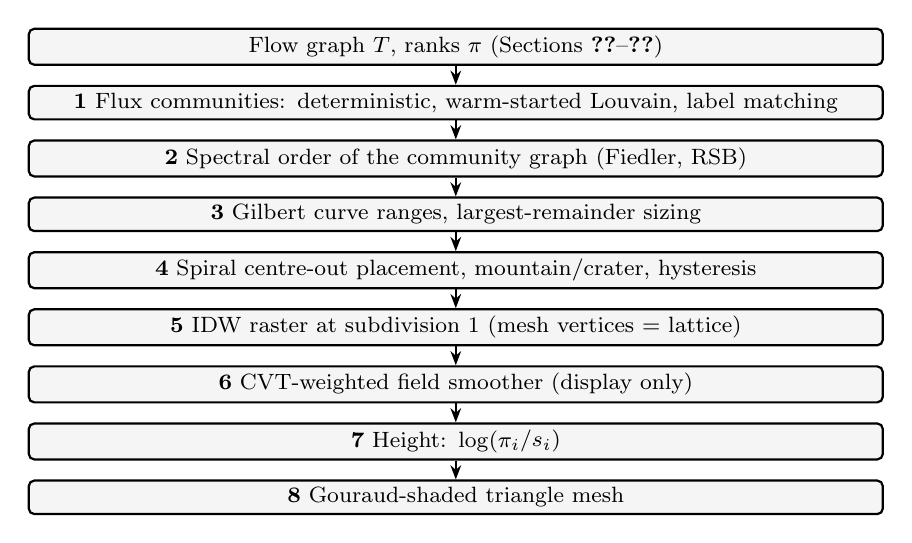
\begin{tikzpicture}[node distance=2.4mm,
  box/.style={draw,rounded corners=2pt,thick,fill=gray!8,text width=0.88\columnwidth,
              align=center,font=\footnotesize,inner sep=2.5pt},
  ar/.style={-{Stealth[length=1.8mm]},thick}]
  \node[box] (f) {Flow graph $T$, ranks $\pi$ (Sections~\ref{Section:model}--\ref{Section:flows})};
  \node[box,below=of f] (s1) {\textbf{1} Flux communities: deterministic, warm-started Louvain, label matching};
  \node[box,below=of s1] (s2) {\textbf{2} Spectral order of the community graph (Fiedler, RSB)};
  \node[box,below=of s2] (s3) {\textbf{3} Gilbert curve ranges, largest-remainder sizing};
  \node[box,below=of s3] (s4) {\textbf{4} Spiral centre-out placement, mountain/crater, hysteresis};
  \node[box,below=of s4] (s5) {\textbf{5} IDW raster at subdivision 1 (mesh vertices = lattice)};
  \node[box,below=of s5] (s6) {\textbf{6} CVT-weighted field smoother (display only)};
  \node[box,below=of s6] (s7) {\textbf{7} Height: $\log(\pi_i/s_i)$};
  \node[box,below=of s7] (s8) {\textbf{8} Gouraud-shaded triangle mesh};
  \foreach \a/\b in {f/s1,s1/s2,s2/s3,s3/s4,s4/s5,s5/s6,s6/s7,s7/s8} \draw[ar] (\a) -- (\b);
\end{tikzpicture}
\caption{The \FS\ pipeline, in the order it runs per frame. Steps 1--4 are placement, steps 5--8 display; display-only changes redraw cached frames without re-running the model. Step 7 sets the vertex values that steps 5--6 interpolate; it is listed where it is defined in the text.}
\label{Figure:pipeline}
\end{figure}

\subsection{Flux-community territories}
\label{Section:louvain}
The community graph is the set of off-diagonal kept edges of $P$ among active stocks, weighted by accumulated raw flow $R$ and symmetrized, $W=R+R^{\mathsf T}$. A two-phase Louvain~\cite{louvain} at resolution 1.0 runs deterministically: nodes are visited in ascending index, ties go to the lowest community id, at most 50 passes per level, and levels aggregate until nothing changes. Communities smaller than 8 stocks merge into their most strongly connected neighbour; those with no neighbour form one ``loose'' pool laid out last; at most 256 communities are kept.

The clustering is refreshed every 5 bars. Three mechanisms keep a community's identity across refreshes. (i) \emph{Warm start}: phase 1 starts from the previous partition rather than from singletons; the very first clustering is refined by warm-starting from its own result until it is a fixed point (at most 4 rounds). (ii) \emph{Matching}: new communities are matched greedily by overlap to old labels, accepting a pair when the Jaccard overlap is at least 0.3 or at least 60\% of the new community lies inside the old one (containment); unmatched communities get fresh labels. (iii) \emph{Order}: matched labels keep their previous layout order. Between refreshes, a newly active stock joins the community of its strongest active neighbour. The first 5 bars only warm up the model.

\subsection{Spectral order of the community graph}
Communities that trade with each other should be adjacent on the lattice. The community graph (summed weights) is ordered by recursive balanced bisection: compute the Fiedler vector~\cite{fiedler} of the normalized Laplacian $L_{\mathrm{sym}}=I-D^{-1/2}WD^{-1/2}$~\cite{chung} by 500 power iterations on $2I-L_{\mathrm{sym}}$ with the trivial vector deflated, sort the communities by it, and split where the cumulative \emph{stock} count is nearest half, as in RSB~\cite{rsb}; disconnected sets fall back to their components. Sign alone orients each recursive call arbitrarily (a chain A--B--C--D can come out BADC), so after recursing each half is reversed if needed so that its end nearer the other half is the one more strongly connected to it (\emph{half-orientation}).

\subsection{Generalized Hilbert curve and territory sizing}
The lattice cells are ordered by the generalized Hilbert (``gilbert2d'') curve~\cite{hilbert,gilbert}, which visits every cell of an arbitrary $n\times m$ rectangle once, with consecutive cells at Chebyshev distance 1. Each community takes a consecutive range of the curve in spectral order, so it owns one contiguous region. With $A$ active stocks and $C\ge A$ cells, community $g$ with $a_g$ stocks gets $c_g=a_g$ cells plus its largest-remainder share of the $C-A$ spare cells (ties to the lower id), so the areas are proportional to the stock counts and sum exactly to $C$.

\subsection{Spiral placement, mountains and craters, hysteresis}
Inside a territory the cells form a spiral: they are sorted by ring $\lfloor\sqrt{d^2}\rfloor$ around the territory centre, then by angle $\mathrm{atan2}(dy,dx)$ from $-\pi$, then by index, so consecutive slots are neighbours. Stocks are ranked by a smoothed value $s=(1-\beta)v+\beta s_{\mathrm{prev}}$ ($\beta=0.5$) of the displayed quantity $v$ and take the slots in rank order. A territory is a \emph{mountain} if its median $s$ is at or above the median over all active stocks, and a \emph{crater} otherwise; a mountain puts its highest values nearest the centre, a crater its lowest. The outer $c_g-a_g$ slots stay empty and form seams between territories.

\emph{Hysteresis}: a stock keeps its previous cell if it was active last frame, is in the same community, the lattice size is unchanged, that cell still lies inside its territory, and the cell's slot in the current spiral is within $\max(2,\,0.15\,c_g)$ slots of its new slot. Conflicts resolve in rank order: kept cells first, then the ideal slot if free, then the nearest free slot of the territory.

\subsection{IDW at subdivision 1}
The raster has $(n\,s)\times(m\,s)$ pixels with subdivision $s=1$ by default, so the raster vertices \emph{are} the lattice points and become the mesh vertices. Each pixel is the Shepard~\cite{shepard} interpolant $z=\sum_i w_i h_i/\sum_i w_i$ with $w_i=d_i^{-2}$ over occupied cells within radius 3 cells; a pixel on a stock takes its value exactly, and a pixel with no stock in range takes its nearest stock, found by one multi-source breadth-first search per frame.

\subsection{CVT-weighted field smoother}
IDW leaves a ``Mexican hat'': an isolated peak is surrounded by a ring that dips toward the background. The display smoother is a Lloyd-style relaxation~\cite{lloyd,cvt} with the pixels as generators. A pixel's Voronoi cell is its square, so its neighbourhood is the $3\times3$ block with area weights 1 (centre and edge neighbours) and 0.5 (diagonals). With density $\rho=\varepsilon+|z|$, $\varepsilon=0.1\cdot\mathrm{P90}(|z|)$, each Jacobi iteration sets
\begin{equation}
z'=(1-\lambda)\,z+\lambda\,\frac{\sum a\rho z}{\sum a\rho},
\end{equation}
with 12 iterations and $\lambda=0.6$. Tall neighbours pull a pixel toward them, which fills the ring without moving any stock. On a $15\times15$ test lattice with one spike of 10 on a background of 1 and its 8-neighbour ring at 0, the ring dip (far background minus the ring minimum) is 0.358 without smoothing, $-0.031$ with a Gaussian of $\sigma=1$ cell and $-0.477$ with the CVT smoother. The negative values mean the ring ends \emph{above} the background: the smoother overshoots into a halo, and it does not conserve the mean height. The smoothing is for the eye only; the ranking table, the tooltips and the API always show exact, unsmoothed values.

\subsection{Height: \texorpdfstring{$\pi$}{pi} relative to size}
Raw $\pi$ is dominated by size, since the largest names carry the largest flows. The landscape height under the \MR\ preset is therefore $\log(\pi_i/s_i)$, where $s_i$ is stock $i$'s size share (its trailing median dollar volume over the sum over active stocks): it shows how much more money a stock attracts than its size predicts, balanced around 0. With uniform $s_i=1/N$ this reduces to the score $\log(\pi_i N)$, the height used for Figure~\ref{Figure:landscape}. The value also drives the spiral ordering and the mountain/crater rule, so changing it re-places the stocks; the ranking itself is always $\pi$.

\subsection{Gouraud-shaded mesh}
Each lattice quad is split into two triangles with a fixed index buffer, so per frame only the vertex heights change. Vertex colours come from a diverging map symmetric around 0 (red for inflow, blue for outflow), scaled robustly by the 90th percentile of $|z|$ and soft-clipped by $\tanh$, and each triangle is Gouraud-shaded~\cite{gouraud} with relief lighting. The strongest flux arcs and the user's portfolio, as rings, are drawn on top.

%% ------------------------------------------------------------------
\section{Results on real data}
\label{Section:results}

\paragraph{Data} The universe is the 10,000-ticker liquidity snapshot with daily (1d) bars from the lake, replayed offline; on the latest bar, 2026-10-01, 6,188 stocks are active under the \$1M liquidity floor.

\paragraph{Top of the ranking} Table~\ref{Table:top} lists the ten highest MarketRank scores $\pi N$. The top is the large-cap semiconductor and technology complex, together with TSLA, META and one leveraged inverse semiconductor ETF (SOXS). Below them come AMZN (\#13), GOOGL (\#18), AVGO (\#21), QQQ (\#24) and SPY (\#25). This is what the model should produce: the names that send and receive the most dollars, and that receive a large share of what their large counterparties pass on, accumulate the most rank.

\begin{table}[t]
\centering
\caption{Top 10 by MarketRank score $\pi N$ (1 = average) on 2026-10-01, replay, 6,188 active stocks.}
\label{Table:top}
\small\setlength{\tabcolsep}{4pt}
\begin{tabular}{rllr}
\toprule
\# & Ticker & Sector & $\pi N$\\
\midrule
1 & MU & Inf.\ Technology & 387.43\\
2 & SNDK & Inf.\ Technology & 373.25\\
3 & NVDA & Inf.\ Technology & 245.87\\
4 & TSLA & Cons.\ Discretionary & 214.61\\
5 & SOXS & ETF/Fund & 203.70\\
6 & META & Comm.\ Services & 188.95\\
7 & MSFT & Inf.\ Technology & 157.76\\
8 & AAPL & Inf.\ Technology & 153.02\\
9 & AMD & Inf.\ Technology & 151.37\\
10 & INTC & Inf.\ Technology & 123.40\\
\bottomrule
\end{tabular}
\end{table}

\begin{figure*}[t]
\centering
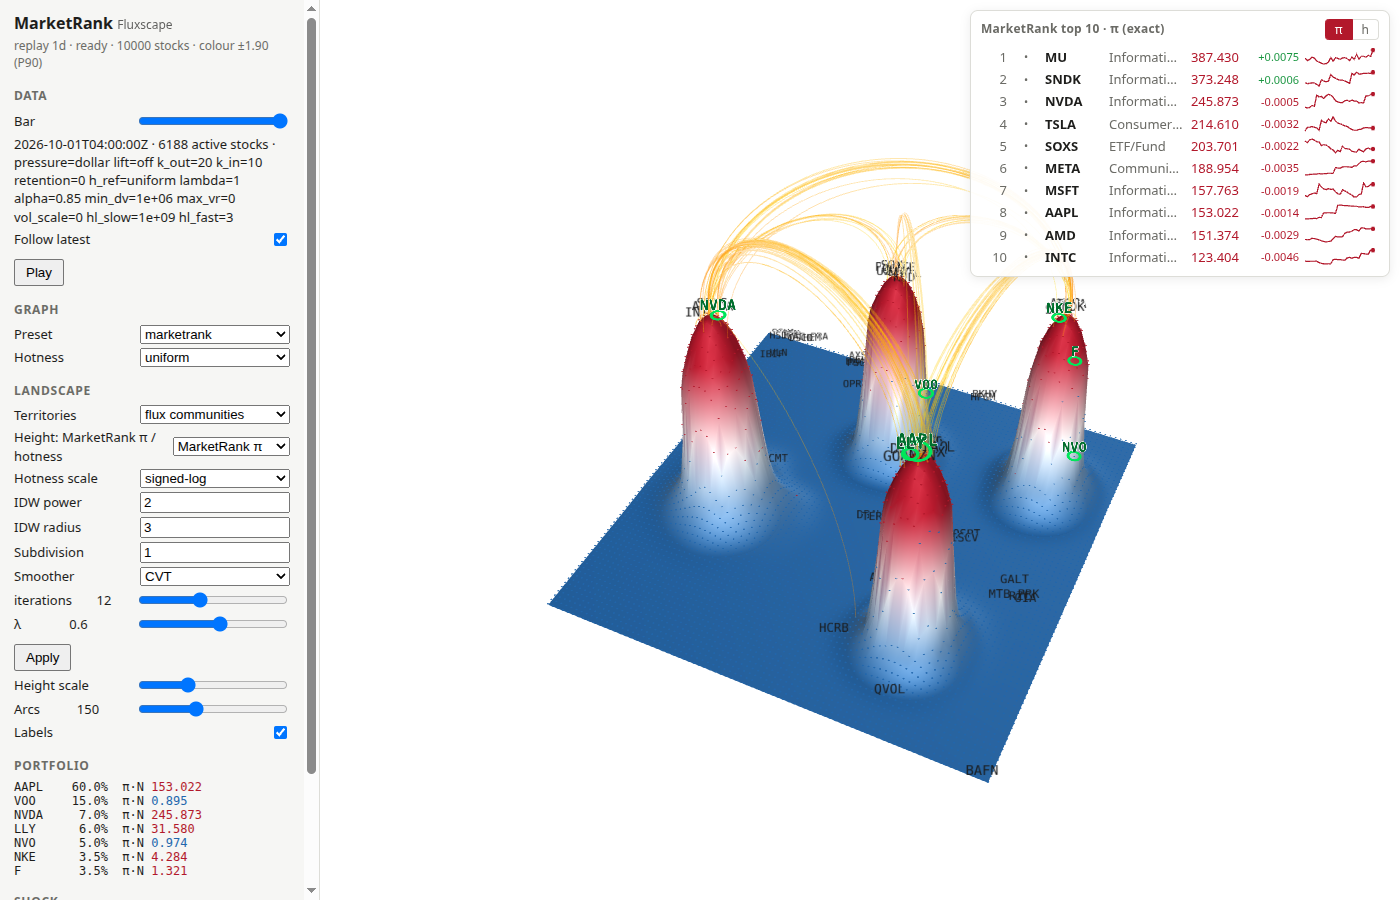
\includegraphics[width=0.92\textwidth,keepaspectratio]{figs/fluxscape-cvt.png}
\caption{\FS\ on real data, 2026-10-01, 6,188 active stocks, \MR\ preset, flux-community territories, IDW (power 2, radius 3, subdivision 1) and the CVT smoother (12 iterations, $\lambda=0.6$). Height here is $\log(\pi_i N)$. The table at the top right is the exact top 10 by $\pi N$ with sparklines of recent history; green rings are portfolio holdings. This screenshot predates the heartbeat redefinition: its pulse column shows $\Delta\log\pi$.}
\label{Figure:landscape}
\end{figure*}
% TODO(fig-final): replace figs/fluxscape-cvt.png with the screenshot of the final UI (controller will supply it).
% TODO(fig): add the README's graph-slice figure once docs/img/marketrank-slice.svg exists,
% converted to PDF (e.g. figs/marketrank-slice.pdf); it does not exist yet.

\paragraph{Contrast with hotness} The engine's earlier ``money-flow'' preset reads a different quantity, hotness relative to size, $h_i=\pi_i/\pi^{\mathrm{ref}}_i-1$ with $\pi^{\mathrm{ref}}$ proportional to trailing median dollar volume, on a chain in which net buyers retain part of their inflow. Its top 10 on the same data are TNON, KOD, DFNS, NFEGP, SOAR, BNAI, WETO, LHSW, AGEN and GRML: all small, all without a known sector. Dividing by size rewards any stock whose flow is large relative to a small denominator, so a single volume spike in an illiquid name outranks steady flow in a mega-cap. The ratio is informative, but as a primary ranking it is dominated by noise in the smallest names, which is why \MR\ ranks by $\pi$ and uses size only for the landscape height.

\paragraph{Evaluation} The harness runs the pipeline over the last 60 of 251 daily bars (10,000 nodes) for a grid of configurations and reports, per configuration: the \emph{floor share} (fraction of active stocks at the teleport floor), the Gini coefficient of $\pi$, \emph{sector coherence} (share of off-diagonal raw edge weight between stocks of the same known sector), \emph{structure gain} ($1-$ Spearman of $\pi$ against inflow share; near 0 means the chain has collapsed to plain inflow), and the information coefficient (IC: the mean per-bar Spearman correlation with the next bar's return, with its $t$-statistic) of the $+1$-bar forecast score and of hotness $h$. Table~\ref{Table:eval} gives the result. Here ``legacy'' is the first milestone (dollar pressure, no pruning of inbound edges, no retention); +A to +E switch on, one at a time, relative pressure, excess-over-gravity lift, $k_{\mathrm{in}}=10$, size or long-run hotness references, and retention; ``defaults'' has them all; ``money-flow'' is dollar pressure with two-sided pruning and retention. The \MR\ preset was added to the grid after this run and has not yet been evaluated.

\begin{table*}[t]
\centering
\caption{Evaluation grid on real data: last 60 of 251 daily bars, 10,000 nodes, 22 threads. IC is the mean per-bar Spearman correlation with the next bar's close-to-close return; $t$ its $t$-statistic. The last column is the mean core frame time.}
\label{Table:eval}
\small\setlength{\tabcolsep}{5pt}
\begin{tabular}{lrrrrrrrrr}
\toprule
Configuration & Floor & Gini & Coherence & Structure & IC(score) & $t$ & IC($h$) & $t$ & ms/frame\\
\midrule
legacy             & 0.947 & 0.847 & 0.378 & 0.642 & $+0.0093$ & $+1.94$ & $-0.0240$ & $-3.95$ & 186.9\\
+A relative        & 0.949 & 0.843 & 0.000 & 0.643 & $+0.0146$ & $+5.04$ & $-0.0471$ & $-10.98$ & 189.0\\
+B excess          & 0.929 & 0.843 & 0.358 & 0.591 & $+0.0096$ & $+1.83$ & $-0.0267$ & $-4.27$ & 113.9\\
+C $k_{\mathrm{in}}=10$ & 0.850 & 0.840 & 0.365 & 0.419 & $+0.0099$ & $+1.72$ & $-0.0274$ & $-4.30$ & 247.0\\
+D size            & 0.947 & 0.847 & 0.378 & 0.642 & $+0.0093$ & $+1.94$ & $-0.0043$ & $-0.53$ & 190.1\\
+D longrun         & 0.947 & 0.847 & 0.378 & 0.642 & $+0.0093$ & $+1.94$ & $+0.0031$ & $+0.81$ & 284.7\\
+E retention       & 0.001 & 0.760 & 0.378 & 0.628 & $-0.0095$ & $-0.72$ & $-0.0243$ & $-1.18$ & 194.9\\
defaults           & 0.001 & 0.743 & 0.224 & 0.429 & $-0.0164$ & $-1.20$ & $-0.0195$ & $-1.30$ & 75.9\\
defaults relative  & 0.002 & 0.728 & 0.125 & 0.318 & $-0.0092$ & $-0.66$ & $-0.0306$ & $-3.54$ & 75.3\\
defaults+longrun   & 0.001 & 0.743 & 0.224 & 0.429 & $-0.0164$ & $-1.20$ & $-0.0041$ & $-0.28$ & 110.2\\
defaults+netflow   & 0.001 & 0.743 & 0.224 & 0.429 & $-0.0164$ & $-1.20$ & $-0.0103$ & $-0.36$ & 71.9\\
money-flow         & 0.001 & 0.732 & 0.360 & 0.508 & $-0.0155$ & $-1.10$ & $-0.0057$ & $-0.91$ & 164.6\\
money-flow+netflow & 0.001 & 0.732 & 0.360 & 0.508 & $-0.0155$ & $-1.10$ & $-0.0136$ & $-0.49$ & 161.1\\
defaults+volscale  & 0.002 & 0.742 & 0.152 & 0.369 & $-0.0203$ & $-1.61$ & $-0.0144$ & $-1.09$ & 72.0\\
money-flow+volscale& 0.002 & 0.747 & 0.254 & 0.493 & $-0.0217$ & $-1.66$ & $-0.0050$ & $-0.79$ & 160.7\\
\bottomrule
\end{tabular}
\end{table*}

The honest reading is as follows. \emph{Structure exists}: with dollar pressure, raw edge weight between stocks of the same sector is 0.36--0.38 of the total, and structure gain is 0.3--0.6 in every configuration, so the pruned multi-hop chain is not just a restatement of who received the most inflow. (Coherence 0.000 under relative pressure alone is an outlier we have not explained.) \emph{Prediction does not}: every IC is at most a few hundredths in magnitude. The largest $|t|$ values belong to configurations without retention, where 85--95\% of stocks sit at the teleport floor, and they have opposite signs for the score and for $h$ (for example $+0.015$ and $-0.047$ under relative pressure), consistent with short-term reversal in a degenerate chain rather than with a usable signal. In the non-degenerate configurations (floor share near 0) only one IC reaches $|t|>2$, the hotness of defaults with relative pressure ($-0.031$, $t=-3.54$), and it is again negative. Open-to-open variants (decide at the close, fill at the next open), also in the log, give the same picture. We read the predictive IC as approximately zero. \MR\ is a description of where estimated money sits, not a return forecast.

\paragraph{Landscape} Figure~\ref{Figure:landscape} shows the real landscape on 2026-10-01 with flux-community territories: four broad mountains, the strongest flux arcs and the portfolio rings. At Louvain resolution 1.0 the real flux graph forms a median of 4 communities (4--5) with modularity 0.13 (0.09--0.25) over 49 re-clusters; it is a weakly modular graph.


\paragraph{Stability} Measured over the real replay (245 landscape frames, 48 re-clusters): between re-clusters the median jump of a stock is 0 cells (p90 also 0) and 85\% of stocks keep their cell on average (96\% on bars where the lattice size is unchanged), against a 13-cell median jump and 4\% kept before hysteresis and spiral ordering. At a re-cluster 39\% keep their cell (median jump 15 cells). Community labels persist for 74\% of stocks per re-cluster (median 76\%, worst 47\%), against about 52\% before the warm start and matching. Mountains and craters stay coherent: the median Spearman correlation of value against distance from the territory centre is 0.98.

\paragraph{Performance} The server is ready to serve about 25\,s after start on the 10,000-ticker replay. A landscape frame takes 10--14\,ms on top of the core step, and a Louvain re-cluster about 35\,ms (in the earlier stability measurement, a median of 28\,ms at resolution 1.0 and 37\,ms at 1.5); only re-cluster frames pay it.

%% ------------------------------------------------------------------
\section{Limitations and future work}
\label{Section:limits}

\paragraph{The flows are inferred} $T$ is an estimate built from simultaneous price and dollar-volume moves (Section~\ref{Section:flows}), not paired transactions. The rank inherits every assumption of Equation~(\ref{eqn:gravity}), and it cannot distinguish a true rotation from two unrelated stocks that moved in opposite directions on the same day.

\paragraph{Teleport floor} Under the \MR\ preset 70.9\% (about 71\%) of active stocks sit at the teleport floor: each source reaches at most 64 of the 256 largest sinks per bar, and two-sided pruning keeps 20 out- and 10 in-edges, so most small stocks never receive kept inflow and hold only teleport mass. The ranking is informative at the top and flat below it.

\paragraph{Leveraged ETFs} Leveraged and inverse ETFs such as SOXS combine large dollar volume with large returns, so they produce large $|\phi|$ and rank high; they are ordinary nodes today, although their flows are partly mechanical.

\paragraph{Planned work}
\begin{itemize}
\item \textbf{13F paired flows.} SEC Form 13F~\cite{sec13f} filings on EDGAR~\cite{edgar} give each institutional manager's quarterly holdings. The per-manager change between quarters (cuts in some names, adds in others) is an \emph{observed} account-level pairing of sources and sinks. Quarterly, delayed and long-only as it is, it can calibrate the bar-level estimate, for example the affinity $a_{ij}$.
\item \textbf{ETF creation and redemption flows}, which move money into or out of a basket of constituents at once.
\item \textbf{Signed order flow} via the Lee--Ready classification~\cite{leeready} of intraday trades, in place of the sign of the bar return.
\item \textbf{Lagged pairing}, so that money sold on one bar can arrive on a later one.
\item \textbf{An observed-flow ingest}, so that $T$ can mix estimated and observed edges.
\item \textbf{Live minute streaming}, extending the replay pipeline to append bars as they close.
\end{itemize}

%% ------------------------------------------------------------------
\section{Conclusion}
\label{Section:conclusion}

\MR\ is a Markov-chain transition-probability solver for money. A stock's score is its stationary probability: the share of the market's estimated dollar flow that settles on it in the steady state of a damped chain. PageRank is the best-known instance of the same idea. The model is small enough to check by hand (the three-stock example) and the engine is fast and deterministic enough to rank 10,000 tickers bit-identically on any thread count. \FS\ makes the result legible as a stable landscape of flux communities. On real data the ranking puts the large-cap semiconductor and technology complex on top and the flow graph shows sector structure, but the evaluated scores have no material predictive power for next-day returns. The flows are inferred; calibrating them against observed pairings, starting with 13F holdings changes, is the most important next step.

\section*{Software availability}
\MR\ is a C++20 program; the model, the evaluation harness and the \FS\ view described here are those of the current implementation.

\bibliography{marketrank}

\end{document}
